\documentclass[a4paper,12pt]{article} %Tipo de documento

%Insercion de paquetes.
\usepackage[utf8]{inputenc}
\usepackage[spanish]{babel}
\usepackage{graphicx} %Inserción de imágenes.
\usepackage[table,xcdraw]{xcolor} %Detecicon de colores.
\usepackage[most]{tcolorbox} %Para el cuadrado del nombre.
\usepackage{fancyhdr} %Estilo de Página.
\usepackage[hidelinks]{hyperref} %Gestion de hypervinculos.
\usepackage{parskip} %Arreglo de la sangría del documento.
\usepackage{geometry}
\usepackage{listings}
\usepackage[T1]{fontenc}
\usepackage[backend=biber]{biblatex}

%Variables para insertar codigo.
\definecolor{codegreen}{rgb}{0,0.6,0}
\definecolor{codegray}{rgb}{0.5,0.5,0.5}
\definecolor{codepurple}{HTML}{59b300}
\definecolor{backcolour}{rgb}{0.95,0.95,0.92}
\lstdefinestyle{mystyle}{
    backgroundcolor=\color{backcolour},
    commentstyle=\color{codegreen},
    keywordstyle=\color{magenta},
    numberstyle=\tiny\color{codegray},
    stringstyle=\color{codepurple},
    basicstyle=\ttfamily\footnotesize,
    breakatwhitespace=false,
    breaklines=true,
    captionpos=b,
    keepspaces=true,
    numbers=left,
    numbersep=5pt,
    showspaces=false,
    showstringspaces=false,
    showtabs=false,
    tabsize=2
    }
    \lstset{style=mystyle}
    %Fin variables de codigo
    %Variables extras.
    \geometry{
        a4paper,
        left=20mm,
        right=20mm,
        top=20mm,
        bottom=20mm,
        headheight=17pt,
        }
        \bibliography{referencias}
        \fancyhf{}
        \pagestyle{fancy}
        \lhead{\Proyecto}
        \rhead{\Nombre}
        \renewcommand{\lstlistingname}{Conjunto de comandos}
        \renewcommand{\labelenumii}{\Roman{enumii}}
        \newlength{\textundbildtextheight}
        \newcommand{\image}[2][1]{\includegraphics[width=#1\textwidth,height=#1\textheight,keepaspectratio]{#2}}

        %=============================================
        \newcommand{\Nombre}{Carlos Sesma Usarralde}
        \newcommand{\Proyecto}{Tarea IV, Despliegue de Aplicaciones Web}
        \definecolor{acentColor}{HTML}{0099ff}
        \definecolor{black}{HTML}{000000}
        \graphicspath{{img/}} %Setting the graphicspath
        \setcounter{tocdepth}{1} % Show sections
        \setcounter{tocdepth}{2} % + subsections
        \setcounter{tocdepth}{3} % + subsubsections

%=============================================
%Incio de documento.
\begin{document}
\cfoot{\thepage}
%Inicio de Portada.
\begin{titlepage}
    \begin{center}
        \huge\textbf{\Proyecto}
    \end{center}
    \hfill{}
    %Línea acent
    {\color{acentColor}\hrule}
    \vfill{}
    \begin{center}
        % \includegraphics[width=0.8\textwidth]{}
    \end{center}
    \vfill{}
    \begin{center}
        {\large{} \Nombre}
    \end{center}
\end{titlepage}
%Fin de portada.
%Inicio índice
\clearpage{}
\tableofcontents{}
\thispagestyle{empty}
\clearpage{}
%Fin del índice
\section{Configuración servidor DHCP en entorno virtualizado}

Para esta practica vamos a instalar el servidor DHCP en un servidor Ubuntu Server y conectaremos a esta un cliente Windows y un cliente Ubuntu.


\subsection{Arrancamos la máquina con una red NAT y una red Bridge}


\includegraphics{00.png}


\subsection{Actualizamos:}
\subsubsection{Paquetes}

\image[1]{01.png}
\subsubsection{Sistema}

\image{02.png}

\subsection{Instalamos `isc-dhcp-server'}
\image{03.png}

Desactivamos la interfaz Bridge y la cambiamos por una red interna

\image{04.png}

(Configuración de red interna)


\includegraphics{07.png}

\subsection{Configuramos el archivo mediante el archivo ubicado en `/etc/dhcp/dhcpd.conf'}


\includegraphics{06.png}

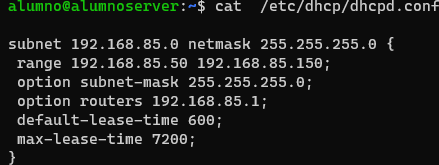
\includegraphics{05.png}



\subsection{Luego definimos como IP del servidor una IP estática que este fuera del rango DHCP}


\includegraphics{09.png}

\image{08.png}

\subsection{Aplicamos la configuración con netplan apply}


\includegraphics{10.png}
\subsubsection{Interfaz levantada y configurada (ens34)}
\image{11.png}

\subsection{Reinciamos el servicio `isc-dhcp-server' usando systemctl}
\image{13.png}


\section{Captura pantalla de configuración servidor e imagen de servicio activo}
\subsection{DHCPD.conf}


\includegraphics{06.png}

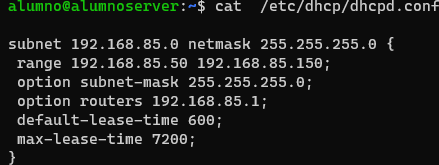
\includegraphics{05.png}
\subsection{Con esto ya tenemos el servicio configurado}
\image{12.png}

\section{Comprobración entrega dirección alquilada a cliente ubuntu}
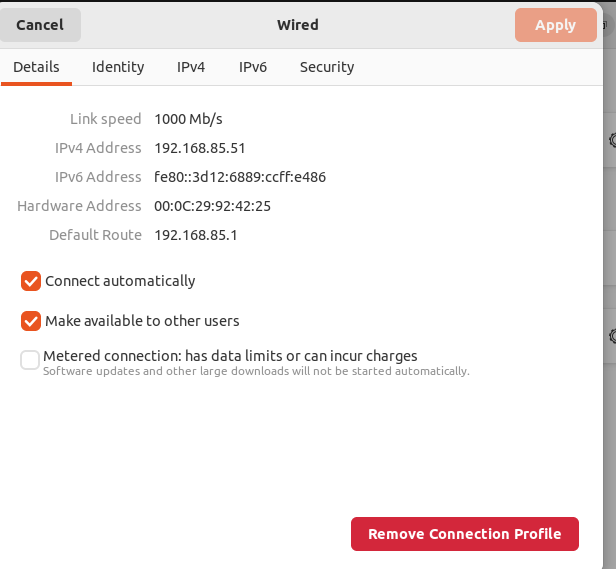
\includegraphics{15.png}


\section{Comprobación entrega dirección a cliente Windows con captura de solicitud de renovación}
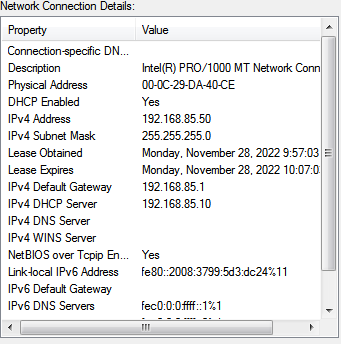
\includegraphics{14.png}


\end{document}
